

The following examples are from papers that study algorithms recovering weaker solution concepts, such as min-max critical points, due to the potential non-existence and the complexity of computing Nash Equilibria. Examples ... were used to demonstrate the failure of convergence of gradient-based algorithms.

\begin{game}\label{ex.daskalakis.d}
A two-player zero-sum game in $1 \times 1$ variables on the interval
$$x_{i1} \in [0,1] \quad \forall i \in \{1, 2\},$$
with the utility function
\begin{align*}
u_{1}\left( x_{1}, x_{2} \right) &= \left( -0.5 + x_{11} \right) \left( -0.5 + x_{21} \right).
\end{align*}
This game was studied by \textcite[Appendix D]{daskalakis.golowich.ea:stay-on-the-ridge}. The game has a value of $0$ and a pure Nash equilibrium at $(x_{11},x_{21}) = (0.5, 0.5)$.
\end{game}

\begin{game}\label{ex.daskalakis.e.1st}
A two-player zero-sum game in $1 \times 1$ variables on the interval
$$x_{i1} \in [0,1] \quad \forall i \in \{1, 2\},$$
with the utility function \cite[Appendix E]{daskalakis.golowich.ea:stay-on-the-ridge}
\begin{align*}
u_{1}\left( x_{1}, x_{2} \right) &= \left(  - 4 x_{11}^{2} + \frac{x_{21}^{4}}{10} + \left(  - 3 x_{11} + x_{21} + \frac{x_{11}^{3}}{20} \right)^{2} \right) e^{\frac{1}{100} \left(  - x_{11}^{2} - x_{21}^{2} \right)}
\end{align*}
The only local min-max equilibrium is $(x_{11},x_{21}) = (0, 0)$. This game was also studied by \textcite{Chinchilla2024,wang2019solvingminimaxoptimizationlocally,zheng.zhu.ea:universal}.
\end{game}


\begin{game}\label{ex.mertikopoulos18.fig1}
A two-player zero-sum game in $1 \times 1$ variables on the interval
$$x_{i1} \in [0,1] \quad \forall i \in \{1,2\}.$$
The utility function is defined by
\begin{align*}
u_{1}\left( x_{1}, x_{2} \right) &= -\left(x_{11}-\frac{1}{2}\right)\left(x_{21}-\frac{1}{2}\right)-\frac{1}{3}e^{-\left(x_{11}-\frac{1}{4}\right)^2-\left(x_{21}-\frac{3}{4}\right)^2}
\end{align*}
\textcite[Fig. 1]{mertikopoulos.lecouat.ea:optimistic} demonstrated divergent behavior of \emph{Mirror Descent} on this non-monotone saddle-point problem. The game has an $\eps$-NE:
\begin{align*}
\mu_1^\star &\approx \delta_{0.38},\\
\mu_2^\star &\approx 0.433\delta_{0} + 0.567\delta_{1}
\end{align*}
achieving a value of $0.247$.
\end{game}

\begin{game}\label{ex.mertikopoulos18.2.2}
A two-player zero-sum game in $1 \times 1$ variables on the interval
$$x_{i1} \in [-1,1] \quad \forall i \in \{1,2\}.$$
The utility function is
\begin{align*}
u_{1}\left( x_{1}, x_{2} \right) = \left( 1 - x_{21}^{2} + x_{21}^{4} x_{11}^{2} \right) \left( -1 - x_{11}^{2} - x_{21}^{2} x_{11}^{4} \right)
\end{align*}
This non-monotone saddle-point problem was studied by \textcite[(2.2)]{mertikopoulos.lecouat.ea:optimistic}. The unique saddle point is $x^\star = (0,0)$.
\end{game}


\noindent
\begin{minipage}[c]{0.6\textwidth}
\begin{game}\label{ex.razaviyayn20.5.1}
A two-player zero-sum game in $1 \times 1$ variables on the intervals
\begin{align*}
    x_1 &\in [-1,1]\\
    x_2 &\in [-2\pi, 2\pi]
\end{align*}
with the utility function \cite[Example~1]{razaviyayn.huang.ea:nonconvex}
\begin{align*}
u_{1}\left( x_{1}, x_{2} \right) &=  - \cos\left( x_{21} \right) + 0.2 x_{11} x_{21}
\end{align*}
The game has the $\epsilon$-NE:
\begin{align*}
\mu_1^\star &= 0.5\delta_{ -1 } + 0.5\delta_{ 1 }, \\
\mu_2^\star &= 0.5\delta_{ -2\pi } + 0.5\delta_{ 2\pi }.
\end{align*}

\end{game}
\strut
\end{minipage}
\hfill
\begin{minipage}[c]{0.35\textwidth}
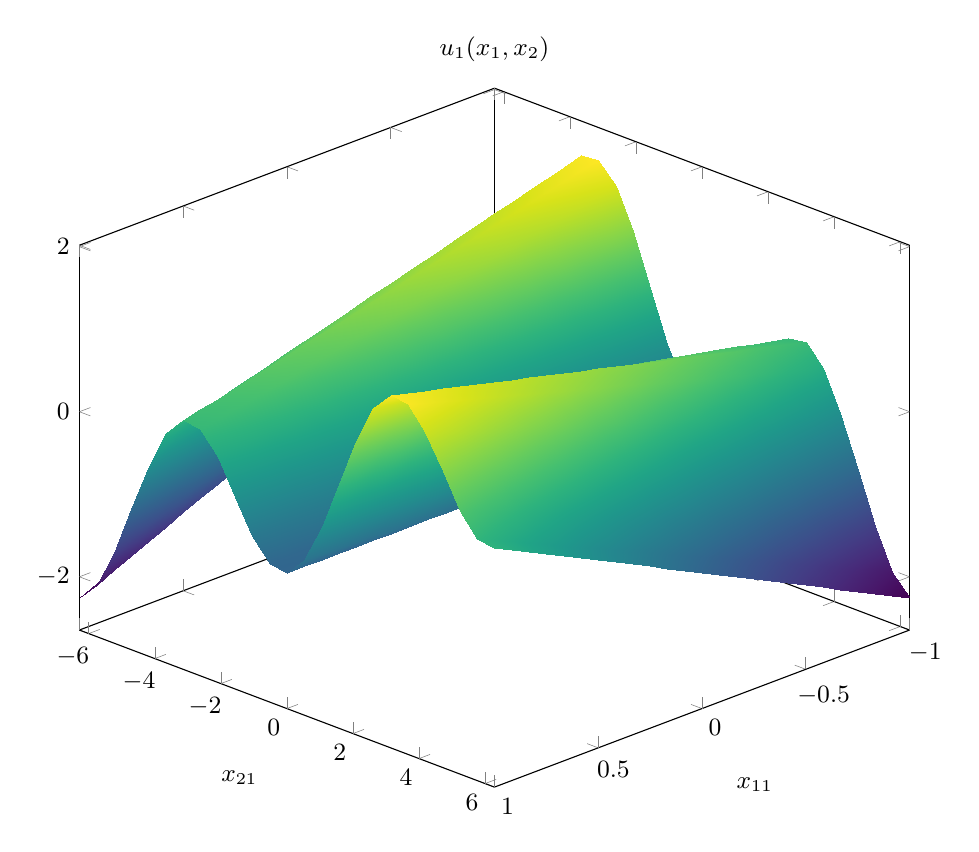
\begin{tikzpicture}
\begin{axis}[
    font=\small,
    domain=-1:1,
    y domain=-6.28318:6.28318,
    xlabel=$x_{11}$,
    ylabel=$x_{21}$,
    title={$u_1(x_1,x_2)$},
    colormap/viridis,
    view={135}{30},
    mesh/ordering=y varies,
    width=\textwidth,
]
\addplot3[
    surf,
    shader=interp,
]
{-cos(deg(y))+0.2*x*y};
\end{axis}
\end{tikzpicture}
\end{minipage}

\begin{game}\label{ex.razaviyayn20.5.3}
A two-player zero-sum game in $1 \times 1$ variables on the interval
\begin{align*}
    x_i &\in [-1,1] \quad \forall i \in \{1,2\}
\end{align*}
with the utility function \cite[Example~3]{razaviyayn.huang.ea:nonconvex}
\begin{align*}
u_{1}\left( x_{1}, x_{2} \right) &= 2 x_{11} x_{21} - x_{21}^{2} + x_{11}^{3}
\end{align*}
The game has the mixed $\epsilon$-NE:
\begin{align*}
\mu_1^\star &\approx \frac{1}{3}\delta_{1} + \frac{2}{3}\delta_{-0.5}, \\
\mu_2^\star &\approx \frac{5}{16}\delta_{1} + \frac{11}{16}\delta_{-1}.
\end{align*}
\end{game}

\begin{game}\label{ex.zheng23.convex.nonconcave}
A two-player zero-sum game in $1 \times 1$ variables on the interval
\begin{align*}
    x_i &\in [-1,1] \quad \forall i \in \{1,2\}
\end{align*}
with utility function given by
\begin{align*}
u_{1}\left( x_{1}, x_{2} \right) &=  - 2 x_{11}^{2} - 4 x_{11} x_{21} + x_{21}^{2} - \frac{4}{3} x_{21}^{3} + \frac{1}{4} x_{21}^{4}
\end{align*}
This example was studied by \textcite[Convex-Nonconcave Example]{zheng.zhu.ea:universal} and also \textcite{Chinchilla2024, pmlr-v89-adolphs19a}.
\end{game}

\begin{game}\label{ex.zheng23.kl.nonconcave}
A two-player zero-sum game in $1 \times 1$ variables on the interval
\begin{align*}
    x_i &\in [-1,1] \quad \forall i \in \{1,2\}
\end{align*}
with utility function \cite[KŁ-Nonconcave Example]{zheng.zhu.ea:universal} given by
\begin{align*}
u_{1}\left( x_{1}, x_{2} \right) &=  - x_{11}^{2} + 4 x_{21}^{2} + 10 \sin^{2}\left( x_{21} \right) - 3 \sin^{2}\left( x_{21} \right) \sin^{2}\left( x_{11} \right)
\end{align*}
This game has the pure NE $x^\star=(0,0)$.
\end{game}

\begin{game}\label{ex.zheng23.bilinearly.coupled.minimax}
A two-player zero-sum game in $1 \times 1$ variables on the interval
\begin{align*}
    x_i &\in [-4,4] \quad \forall i \in \{1,2\}
\end{align*}
with utility function \cite[Bilinearly-coupled Minimax]{zheng.zhu.ea:universal} given by
\begin{align*}
u_1(x_1, x_2) = - f(x_{11}) - Ax_{11}x_{21} + f(x_{21})
\end{align*}
where $f(z)=(z + 1)(z - 1)(z + 3)(z - 3)$. This example was also studied by \textcite{Grimmer2023}.
\end{game}

\begin{game}\label{ex.zheng23.forsaken}
A two-player zero-sum game in $1 \times 1$ variables on the interval
\begin{align*}
    x_i &\in [-1.5,1.5] \quad \forall i \in \{1,2\}
\end{align*}
with utility function \cite[“Forsaken” example]{zheng.zhu.ea:universal} given by
\begin{align*}
u1(x, y) = - x_{11}(x_{21}-0.45) - \phi(x_{11}) + \phi(x_{21})
\end{align*}
where $\phi(z) = \frac{1}{4}z^2 - \frac{1}{2}  z^4 + \frac{1}{6}z^6$. This problem was also studied by \textcite[Example~5.2]{pmlr-v139-hsieh21a}. The game has the mixed $\epsilon$-NE:
\begin{align*}
\mu_1^\star &= 0.5\delta_{ -1.31 } + 0.5\delta_{ 1.31 },\\
\mu_2^\star &= 0.328\delta_{ -1.31 } + 0.672\delta_{ 1.31 }.
\end{align*}
\end{game}
